% Created by tikzDevice version 0.11 on 2018-04-11 18:30:52
% !TEX encoding = UTF-8 Unicode
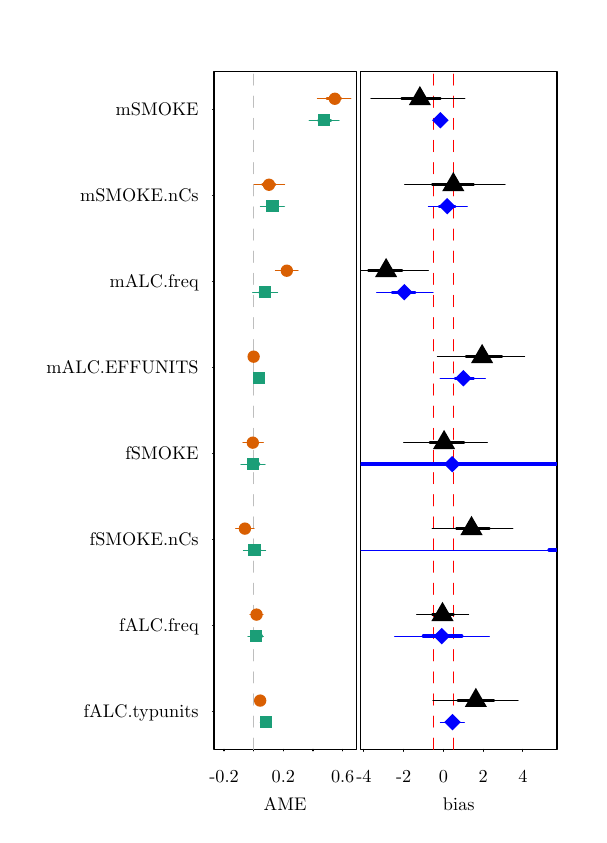
\begin{tikzpicture}[x=1pt,y=1pt]
\definecolor{fillColor}{RGB}{255,255,255}
\path[use as bounding box,fill=fillColor,fill opacity=0.00] (0,0) rectangle (199.17,284.53);
\begin{scope}
\path[clip] (  0.00,  0.00) rectangle (199.17,284.53);
\definecolor{drawColor}{RGB}{0,0,0}

\path[draw=drawColor,line width= 0.4pt,line join=round,line cap=round] ( 70.94, 23.76) -- (113.83, 23.76);

\path[draw=drawColor,line width= 0.4pt,line join=round,line cap=round] ( 70.94, 23.76) -- ( 70.94, 23.25);

\path[draw=drawColor,line width= 0.4pt,line join=round,line cap=round] ( 81.67, 23.76) -- ( 81.67, 23.25);

\path[draw=drawColor,line width= 0.4pt,line join=round,line cap=round] ( 92.39, 23.76) -- ( 92.39, 23.25);

\path[draw=drawColor,line width= 0.4pt,line join=round,line cap=round] (103.11, 23.76) -- (103.11, 23.25);

\path[draw=drawColor,line width= 0.4pt,line join=round,line cap=round] (113.83, 23.76) -- (113.83, 23.25);

\node[text=drawColor,anchor=base,inner sep=0pt, outer sep=0pt, scale=  0.66] at ( 70.94, 11.88) {-0.2};

\node[text=drawColor,anchor=base,inner sep=0pt, outer sep=0pt, scale=  0.66] at ( 92.39, 11.88) {0.2};

\node[text=drawColor,anchor=base,inner sep=0pt, outer sep=0pt, scale=  0.66] at (113.83, 11.88) {0.6};

\path[draw=drawColor,line width= 0.4pt,line join=round,line cap=round] ( 67.32, 23.76) --
	(118.71, 23.76) --
	(118.71,268.69) --
	( 67.32,268.69) --
	( 67.32, 23.76);
\end{scope}
\begin{scope}
\path[clip] (  0.00,  0.00) rectangle (119.50,284.53);
\definecolor{drawColor}{RGB}{0,0,0}

\node[text=drawColor,anchor=base,inner sep=0pt, outer sep=0pt, scale=  0.66] at ( 93.01,  1.58) {AME};
\end{scope}
\begin{scope}
\path[clip] ( 67.32, 23.76) rectangle (118.71,268.69);
\definecolor{drawColor}{RGB}{190,190,190}

\path[draw=drawColor,line width= 0.4pt,dash pattern=on 4pt off 4pt ,line join=round,line cap=round] ( 81.67, 23.76) -- ( 81.67,268.69);
\definecolor{fillColor}{RGB}{27,158,119}

\path[fill=fillColor] (104.84,248.85) --
	(109.29,248.85) --
	(109.29,253.30) --
	(104.84,253.30) --
	cycle;

\path[fill=fillColor] ( 86.28,217.78) --
	( 90.74,217.78) --
	( 90.74,222.23) --
	( 86.28,222.23) --
	cycle;

\path[fill=fillColor] ( 83.47,186.71) --
	( 87.93,186.71) --
	( 87.93,191.17) --
	( 83.47,191.17) --
	cycle;

\path[fill=fillColor] ( 81.42,155.65) --
	( 85.87,155.65) --
	( 85.87,160.10) --
	( 81.42,160.10) --
	cycle;

\path[fill=fillColor] ( 79.22,124.58) --
	( 83.67,124.58) --
	( 83.67,129.03) --
	( 79.22,129.03) --
	cycle;

\path[fill=fillColor] ( 79.74, 93.51) --
	( 84.19, 93.51) --
	( 84.19, 97.97) --
	( 79.74, 97.97) --
	cycle;

\path[fill=fillColor] ( 80.39, 62.45) --
	( 84.85, 62.45) --
	( 84.85, 66.90) --
	( 80.39, 66.90) --
	cycle;

\path[fill=fillColor] ( 83.77, 31.38) --
	( 88.23, 31.38) --
	( 88.23, 35.84) --
	( 83.77, 35.84) --
	cycle;
\definecolor{drawColor}{RGB}{27,158,119}

\path[draw=drawColor,line width= 1.2pt,line join=round,line cap=round] (105.05,251.07) -- (109.54,251.07);

\path[draw=drawColor,line width= 1.2pt,line join=round,line cap=round] ( 86.81,220.01) -- ( 90.34,220.01);

\path[draw=drawColor,line width= 1.2pt,line join=round,line cap=round] ( 83.80,188.94) -- ( 87.52,188.94);

\path[draw=drawColor,line width= 1.2pt,line join=round,line cap=round] ( 82.99,157.87) -- ( 84.40,157.87);

\path[draw=drawColor,line width= 1.2pt,line join=round,line cap=round] ( 79.95,126.81) -- ( 83.44,126.81);

\path[draw=drawColor,line width= 1.2pt,line join=round,line cap=round] ( 80.46, 95.74) -- ( 83.79, 95.74);

\path[draw=drawColor,line width= 1.2pt,line join=round,line cap=round] ( 82.25, 64.67) -- ( 84.44, 64.67);

\path[draw=drawColor,line width= 1.2pt,line join=round,line cap=round] ( 85.12, 33.61) -- ( 86.79, 33.61);

\path[draw=drawColor,line width= 0.4pt,line join=round,line cap=round] (101.69,251.07) -- (112.56,251.07);

\path[draw=drawColor,line width= 0.4pt,line join=round,line cap=round] ( 84.12,220.01) -- ( 92.79,220.01);

\path[draw=drawColor,line width= 0.4pt,line join=round,line cap=round] ( 81.26,188.94) -- ( 90.27,188.94);

\path[draw=drawColor,line width= 0.4pt,line join=round,line cap=round] ( 81.96,157.87) -- ( 85.31,157.87);

\path[draw=drawColor,line width= 0.4pt,line join=round,line cap=round] ( 77.02,126.81) -- ( 85.79,126.81);

\path[draw=drawColor,line width= 0.4pt,line join=round,line cap=round] ( 77.95, 95.74) -- ( 85.96, 95.74);

\path[draw=drawColor,line width= 0.4pt,line join=round,line cap=round] ( 79.59, 64.67) -- ( 85.19, 64.67);

\path[draw=drawColor,line width= 0.4pt,line join=round,line cap=round] ( 84.05, 33.61) -- ( 88.04, 33.61);
\definecolor{fillColor}{RGB}{217,95,2}

\path[fill=fillColor] (111.00,258.84) circle (  2.23);

\path[fill=fillColor] ( 87.19,227.77) circle (  2.23);

\path[fill=fillColor] ( 93.64,196.71) circle (  2.23);

\path[fill=fillColor] ( 81.65,165.64) circle (  2.23);

\path[fill=fillColor] ( 81.35,134.57) circle (  2.23);

\path[fill=fillColor] ( 78.50,103.51) circle (  2.23);

\path[fill=fillColor] ( 82.70, 72.44) circle (  2.23);

\path[fill=fillColor] ( 84.01, 41.37) circle (  2.23);
\definecolor{drawColor}{RGB}{217,95,2}

\path[draw=drawColor,line width= 1.2pt,line join=round,line cap=round] (108.12,258.84) -- (113.12,258.84);

\path[draw=drawColor,line width= 1.2pt,line join=round,line cap=round] ( 84.87,227.77) -- ( 89.41,227.77);

\path[draw=drawColor,line width= 1.2pt,line join=round,line cap=round] ( 92.07,196.71) -- ( 95.46,196.71);

\path[draw=drawColor,line width= 1.2pt,line join=round,line cap=round] ( 80.94,165.64) -- ( 82.20,165.64);

\path[draw=drawColor,line width= 1.2pt,line join=round,line cap=round] ( 79.84,134.57) -- ( 82.94,134.57);

\path[draw=drawColor,line width= 1.2pt,line join=round,line cap=round] ( 77.24,103.51) -- ( 79.90,103.51);

\path[draw=drawColor,line width= 1.2pt,line join=round,line cap=round] ( 82.34, 72.44) -- ( 84.33, 72.44);

\path[draw=drawColor,line width= 1.2pt,line join=round,line cap=round] ( 83.17, 41.37) -- ( 84.61, 41.37);

\path[draw=drawColor,line width= 0.4pt,line join=round,line cap=round] (104.70,258.84) -- (116.81,258.84);

\path[draw=drawColor,line width= 0.4pt,line join=round,line cap=round] ( 81.80,227.77) -- ( 92.83,227.77);

\path[draw=drawColor,line width= 0.4pt,line join=round,line cap=round] ( 89.50,196.71) -- ( 97.74,196.71);

\path[draw=drawColor,line width= 0.4pt,line join=round,line cap=round] ( 80.19,165.64) -- ( 83.25,165.64);

\path[draw=drawColor,line width= 0.4pt,line join=round,line cap=round] ( 77.75,134.57) -- ( 85.18,134.57);

\path[draw=drawColor,line width= 0.4pt,line join=round,line cap=round] ( 75.19,103.51) -- ( 81.81,103.51);

\path[draw=drawColor,line width= 0.4pt,line join=round,line cap=round] ( 80.32, 72.44) -- ( 85.03, 72.44);

\path[draw=drawColor,line width= 0.4pt,line join=round,line cap=round] ( 82.35, 41.37) -- ( 85.76, 41.37);
\end{scope}
\begin{scope}
\path[clip] (  0.00,  0.00) rectangle (199.17,284.53);
\definecolor{drawColor}{RGB}{0,0,0}

\path[draw=drawColor,line width= 0.4pt,line join=round,line cap=round] ( 67.32, 37.49) -- ( 67.32,254.96);

\path[draw=drawColor,line width= 0.4pt,line join=round,line cap=round] ( 67.32, 37.49) -- ( 66.81, 37.49);

\path[draw=drawColor,line width= 0.4pt,line join=round,line cap=round] ( 67.32, 68.56) -- ( 66.81, 68.56);

\path[draw=drawColor,line width= 0.4pt,line join=round,line cap=round] ( 67.32, 99.62) -- ( 66.81, 99.62);

\path[draw=drawColor,line width= 0.4pt,line join=round,line cap=round] ( 67.32,130.69) -- ( 66.81,130.69);

\path[draw=drawColor,line width= 0.4pt,line join=round,line cap=round] ( 67.32,161.76) -- ( 66.81,161.76);

\path[draw=drawColor,line width= 0.4pt,line join=round,line cap=round] ( 67.32,192.82) -- ( 66.81,192.82);

\path[draw=drawColor,line width= 0.4pt,line join=round,line cap=round] ( 67.32,223.89) -- ( 66.81,223.89);

\path[draw=drawColor,line width= 0.4pt,line join=round,line cap=round] ( 67.32,254.96) -- ( 66.81,254.96);

\node[text=drawColor,anchor=base east,inner sep=0pt, outer sep=0pt, scale=  0.66] at ( 61.78, 35.22) {fALC.typunits};

\node[text=drawColor,anchor=base east,inner sep=0pt, outer sep=0pt, scale=  0.66] at ( 61.78, 66.28) {fALC.freq};

\node[text=drawColor,anchor=base east,inner sep=0pt, outer sep=0pt, scale=  0.66] at ( 61.78, 97.35) {fSMOKE.nCs};

\node[text=drawColor,anchor=base east,inner sep=0pt, outer sep=0pt, scale=  0.66] at ( 61.78,128.42) {fSMOKE};

\node[text=drawColor,anchor=base east,inner sep=0pt, outer sep=0pt, scale=  0.66] at ( 61.78,159.48) {mALC.EFFUNITS};

\node[text=drawColor,anchor=base east,inner sep=0pt, outer sep=0pt, scale=  0.66] at ( 61.78,190.55) {mALC.freq};

\node[text=drawColor,anchor=base east,inner sep=0pt, outer sep=0pt, scale=  0.66] at ( 61.78,221.62) {mSMOKE.nCs};

\node[text=drawColor,anchor=base east,inner sep=0pt, outer sep=0pt, scale=  0.66] at ( 61.78,252.68) {mSMOKE};
\end{scope}
\begin{scope}
\path[clip] ( 67.32, 23.76) rectangle (118.71,268.69);
\definecolor{drawColor}{RGB}{0,0,0}

\path[draw=drawColor,line width= 0.4pt,line join=round,line cap=round] ( 67.32,269.56) -- (118.71,269.56);

\path[draw=drawColor,line width= 0.4pt,line join=round,line cap=round] ( 67.32,271.42) -- (118.71,271.42);
\end{scope}
\begin{scope}
\path[clip] (  0.00,  0.00) rectangle (199.17,284.53);
\definecolor{drawColor}{RGB}{0,0,0}

\path[draw=drawColor,line width= 0.4pt,line join=round,line cap=round] (121.49, 23.76) -- (178.93, 23.76);

\path[draw=drawColor,line width= 0.4pt,line join=round,line cap=round] (121.49, 23.76) -- (121.49, 23.05);

\path[draw=drawColor,line width= 0.4pt,line join=round,line cap=round] (135.85, 23.76) -- (135.85, 23.05);

\path[draw=drawColor,line width= 0.4pt,line join=round,line cap=round] (150.21, 23.76) -- (150.21, 23.05);

\path[draw=drawColor,line width= 0.4pt,line join=round,line cap=round] (164.57, 23.76) -- (164.57, 23.05);

\path[draw=drawColor,line width= 0.4pt,line join=round,line cap=round] (178.93, 23.76) -- (178.93, 23.05);

\node[text=drawColor,anchor=base,inner sep=0pt, outer sep=0pt, scale=  0.66] at (121.49, 11.88) {-4};

\node[text=drawColor,anchor=base,inner sep=0pt, outer sep=0pt, scale=  0.66] at (135.85, 11.88) {-2};

\node[text=drawColor,anchor=base,inner sep=0pt, outer sep=0pt, scale=  0.66] at (150.21, 11.88) {0};

\node[text=drawColor,anchor=base,inner sep=0pt, outer sep=0pt, scale=  0.66] at (164.57, 11.88) {2};

\node[text=drawColor,anchor=base,inner sep=0pt, outer sep=0pt, scale=  0.66] at (178.93, 11.88) {4};

\path[draw=drawColor,line width= 0.4pt,line join=round,line cap=round] (120.29, 23.76) --
	(191.25, 23.76) --
	(191.25,268.69) --
	(120.29,268.69) --
	(120.29, 23.76);
\end{scope}
\begin{scope}
\path[clip] (119.50,  0.00) rectangle (199.17,284.53);
\definecolor{drawColor}{RGB}{0,0,0}

\node[text=drawColor,anchor=base,inner sep=0pt, outer sep=0pt, scale=  0.66] at (155.77,  1.58) {bias};
\end{scope}
\begin{scope}
\path[clip] (120.29, 23.76) rectangle (191.25,268.69);
\definecolor{drawColor}{RGB}{255,0,0}

\path[draw=drawColor,line width= 0.4pt,dash pattern=on 4pt off 4pt ,line join=round,line cap=round] (146.62, 23.76) -- (146.62,268.69);

\path[draw=drawColor,line width= 0.4pt,dash pattern=on 4pt off 4pt ,line join=round,line cap=round] (153.80, 23.76) -- (153.80,268.69);
\definecolor{drawColor}{RGB}{0,0,0}

\path[draw=drawColor,line width= 0.4pt,line join=round,line cap=round] (124.06,258.84) -- (158.00,258.84);

\path[draw=drawColor,line width= 0.4pt,line join=round,line cap=round] (136.25,227.77) -- (172.50,227.77);

\path[draw=drawColor,line width= 0.4pt,line join=round,line cap=round] (114.93,196.71) -- (144.80,196.71);

\path[draw=drawColor,line width= 0.4pt,line join=round,line cap=round] (148.02,165.64) -- (179.58,165.64);

\path[draw=drawColor,line width= 0.4pt,line join=round,line cap=round] (135.87,134.57) -- (166.09,134.57);

\path[draw=drawColor,line width= 0.4pt,line join=round,line cap=round] (146.13,103.51) -- (175.34,103.51);

\path[draw=drawColor,line width= 0.4pt,line join=round,line cap=round] (140.53, 72.44) -- (159.33, 72.44);

\path[draw=drawColor,line width= 0.4pt,line join=round,line cap=round] (146.40, 41.37) -- (177.19, 41.37);

\path[draw=drawColor,line width= 1.2pt,line join=round,line cap=round] (135.17,258.84) -- (149.10,258.84);

\path[draw=drawColor,line width= 1.2pt,line join=round,line cap=round] (146.22,227.77) -- (161.13,227.77);

\path[draw=drawColor,line width= 1.2pt,line join=round,line cap=round] (123.12,196.71) -- (135.25,196.71);

\path[draw=drawColor,line width= 1.2pt,line join=round,line cap=round] (158.41,165.64) -- (171.31,165.64);

\path[draw=drawColor,line width= 1.2pt,line join=round,line cap=round] (145.33,134.57) -- (157.64,134.57);

\path[draw=drawColor,line width= 1.2pt,line join=round,line cap=round] (154.93,103.51) -- (166.84,103.51);

\path[draw=drawColor,line width= 1.2pt,line join=round,line cap=round] (146.24, 72.44) -- (153.87, 72.44);

\path[draw=drawColor,line width= 1.2pt,line join=round,line cap=round] (155.44, 41.37) -- (168.45, 41.37);
\definecolor{drawColor}{RGB}{0,0,255}

\path[draw=drawColor,line width= 0.4pt,line join=round,line cap=round] (146.78,251.07) -- (151.23,251.07);

\path[draw=drawColor,line width= 0.4pt,line join=round,line cap=round] (144.81,220.01) -- (158.83,220.01);

\path[draw=drawColor,line width= 0.4pt,line join=round,line cap=round] (126.13,188.94) -- (146.52,188.94);

\path[draw=drawColor,line width= 0.4pt,line join=round,line cap=round] (149.08,157.87) -- (165.37,157.87);

\path[draw=drawColor,line width= 0.4pt,line join=round,line cap=round] (  0.00,126.81) -- (199.17,126.81);

\path[draw=drawColor,line width= 0.4pt,line join=round,line cap=round] (117.15, 95.74) -- (199.17, 95.74);

\path[draw=drawColor,line width= 0.4pt,line join=round,line cap=round] (132.61, 64.67) -- (166.80, 64.67);

\path[draw=drawColor,line width= 0.4pt,line join=round,line cap=round] (149.14, 33.61) -- (157.78, 33.61);

\path[draw=drawColor,line width= 1.2pt,line join=round,line cap=round] (148.24,251.07) -- (150.06,251.07);

\path[draw=drawColor,line width= 1.2pt,line join=round,line cap=round] (148.67,220.01) -- (154.43,220.01);

\path[draw=drawColor,line width= 1.2pt,line join=round,line cap=round] (131.72,188.94) -- (140.00,188.94);

\path[draw=drawColor,line width= 1.2pt,line join=round,line cap=round] (154.44,157.87) -- (161.10,157.87);

\path[draw=drawColor,line width= 1.2pt,line join=round,line cap=round] ( 91.26,126.81) -- (199.17,126.81);

\path[draw=drawColor,line width= 1.2pt,line join=round,line cap=round] (188.40, 95.74) -- (199.17, 95.74);

\path[draw=drawColor,line width= 1.2pt,line join=round,line cap=round] (142.99, 64.67) -- (156.87, 64.67);

\path[draw=drawColor,line width= 1.2pt,line join=round,line cap=round] (151.68, 33.61) -- (155.33, 33.61);
\definecolor{fillColor}{RGB}{0,0,0}

\path[fill=fillColor] (141.73,263.46) --
	(145.73,256.53) --
	(137.73,256.53) --
	cycle;

\path[fill=fillColor] (153.80,232.39) --
	(157.80,225.46) --
	(149.80,225.46) --
	cycle;

\path[fill=fillColor] (129.52,201.33) --
	(133.52,194.40) --
	(125.52,194.40) --
	cycle;

\path[fill=fillColor] (164.21,170.26) --
	(168.21,163.33) --
	(160.21,163.33) --
	cycle;

\path[fill=fillColor] (150.47,139.19) --
	(154.47,132.26) --
	(146.47,132.26) --
	cycle;

\path[fill=fillColor] (160.38,108.13) --
	(164.38,101.20) --
	(156.38,101.20) --
	cycle;

\path[fill=fillColor] (149.89, 77.06) --
	(153.89, 70.13) --
	(145.89, 70.13) --
	cycle;

\path[fill=fillColor] (161.95, 45.99) --
	(165.95, 39.07) --
	(157.95, 39.07) --
	cycle;
\definecolor{fillColor}{RGB}{0,0,255}

\path[fill=fillColor] (146.13,251.07) --
	(149.10,254.04) --
	(152.07,251.07) --
	(149.10,248.10) --
	cycle;

\path[fill=fillColor] (148.63,220.01) --
	(151.60,222.98) --
	(154.57,220.01) --
	(151.60,217.04) --
	cycle;

\path[fill=fillColor] (133.12,188.94) --
	(136.09,191.91) --
	(139.06,188.94) --
	(136.09,185.97) --
	cycle;

\path[fill=fillColor] (154.46,157.87) --
	(157.43,160.84) --
	(160.40,157.87) --
	(157.43,154.90) --
	cycle;

\path[fill=fillColor] (150.41,126.81) --
	(153.38,129.78) --
	(156.35,126.81) --
	(153.38,123.84) --
	cycle;

\path[fill=fillColor] (146.66, 64.67) --
	(149.63, 67.64) --
	(152.60, 64.67) --
	(149.63, 61.70) --
	cycle;

\path[fill=fillColor] (150.53, 33.61) --
	(153.50, 36.58) --
	(156.47, 33.61) --
	(153.50, 30.64) --
	cycle;
\end{scope}
\begin{scope}
\path[clip] (120.29, 23.76) rectangle (191.25,268.69);
\definecolor{drawColor}{RGB}{0,0,0}

\path[draw=drawColor,line width= 0.4pt,line join=round,line cap=round] (120.29,269.56) -- (191.25,269.56);

\path[draw=drawColor,line width= 0.4pt,line join=round,line cap=round] (120.29,271.42) -- (191.25,271.42);
\end{scope}
\end{tikzpicture}
